\documentclass[14pt,a4paper]{extarticle}



\usepackage[utf8]{inputenc}
\usepackage[T2A]{fontenc}
\usepackage{amssymb,amsmath,mathrsfs,amsthm}
\usepackage[russian]{babel}
\usepackage{graphicx}
\usepackage[footnotesize]{caption2}
\usepackage{indentfirst}
\usepackage{multicol}
\usepackage{listings}
\usepackage{float}
\usepackage{url}

\usepackage{enumitem}

%\usepackage[ruled,section]{algorithm}
%\usepackage[noend]{algorithmic}
%\usepackage[all]{xy}
\usepackage{booktabs}
\usepackage{graphicx}
\usepackage[table,xcdraw]{xcolor}
\usepackage{tcolorbox}

%Библиотека для блок-схем
\usepackage{tikz}
\usetikzlibrary{shapes,arrows}

% Параметры страницы
\textheight=24cm
\textwidth=16cm
\oddsidemargin=5mm
\evensidemargin=-5mm
\marginparwidth=36pt
\topmargin=-1cm
\footnotesep=3ex
%\flushbottom
\raggedbottom
\tolerance 3000
% подавить эффект "висячих стpок"
\clubpenalty=10000
\widowpenalty=10000
%\renewcommand{\baselinestretch}{1.1}
\renewcommand{\baselinestretch}{1.5} %для печати с большим интервалом

\newcommand{\angstrom}{\mbox{\normalfont\AA}}

\newtheorem{definition}{Определение} % задаём выводимое слово (для определений)
\newtheorem{example}{Замечание} % задаём выводимое слово (для определений)
\newtheorem{theorem}{Теорема} % задаём выводимое слово (для определений)
\newtheorem{construction}{Конструкция} % задаём выводимое слово (для определений)

\DeclareMathOperator*{\sgn}{sgn}
\DeclareMathOperator*{\var}{var}   
\DeclareMathOperator*{\cov}{cov}
\DeclareMathOperator*{\law}{Law}

\newcommand{\1}{\mathbbm{1}} 
\newcommand{\R}{\mathbb{R}}
\newcommand{\N}{\mathbb{N}}
\newcommand{\Z}{\mathbb{Z}}
\renewcommand{\P}{\mathbb{P}}
\newcommand{\E}{\mathbb{E}}

\newcommand{\independent}{\perp\!\!\!\!\perp}


\newcommand\cA{{\cal A}}
\newcommand\cE{{\cal E}}
\newcommand\cC{{\cal C}}
\newcommand\cF{{\cal F}}
\newcommand\cG{{\cal G}}
\newcommand\cK{{\cal K}}
\newcommand\cL{{\cal L}}
\newcommand\cB{{\cal B}}
\newcommand\cN{{\cal N}}
\newcommand\cM{{\cal M}}
\newcommand\cX{{\cal X}}
\newcommand\cD{{\cal D}}
\newcommand\cR{{\cal R}}
\newcommand\cP{{\cal P}}
\newcommand\cQ{{\cal Q}}
\newcommand\cS{{\cal S}}
\newcommand\cT{{\cal T}}
\newcommand\cV{{\cal V}}
\newcommand\cZ{{\cal Z}}

\newcommand{\textProposition}    {Предложение}

\begin{document}

\begin{center}

{Всеволод Заостровский, 409 группа}\\
{\bfseries Отчёт по задаче "Полиномиальная интерполяция".\\}
\vspace{1cm}

\end{center}

\section{Постановка задачи и теоретическая справка.}
Пусть задана дискретная функция $y_i = f(x_i)$, $i = 0, 1, 2, . . . n - 1$.
Требуется построить алгебраичекий полиноном $P_{n-1}(x)$ степени $n - 1$, удовлетворяющий условиям:

\begin{equation}
    P_{n-1}(x_i) = y_i, i = 0, 1, 2, . . . , n - 1.
\end{equation}

Такой полином называется интерполяционным. Его коэффициенты могут 
быть найдены из решения следующей системы линейных алгебраических
уравнений относительно неизвестных $a_0, a_1, ..., a_{n-1}$:

\begin{equation*}
    \begin{cases}
    a_0 + a_1 x_0 + \ldots + a_{n-1} x^{n-1}_0 = y_0 \\
    a_0 + a_1 x_1 + \ldots + a_{n-1} x^{n-1}_1 = y_1 \\
    \ldots \\
    a_0 + a_1 x_{n-1} + \ldots + a_{n-1} x^{n-1}_{n-1} = y_{n-1} $ $
    \end{cases}
\end{equation*}

Система имеет единственное решение, т.к. ее определителем является определитель Ван дер Монда 
(отличен от нуля в случае $x_i \neq x_j$ , $i \neq j$). Однако,
построение полинома $P_{n-1}(x)$ через явное вычисление его коэффициентов
приводит к катастрофической потере точности уже при $n \approx 20 / 50$. 
Поэтому обычно для расчетов используют запись интерполяционного полинома
в форме Лагранжа:
\begin{equation*}
    P_{n-1}(x) = L_n(x) = \sum\limits_{i=0}^{n-1} y_i \Phi_i(x), \; \Phi_i(x) = \prod\limits_{j \neq i} \frac{x - x_j}{x_i - x_j}
\end{equation*}

\section{Описание программы.}

В классе $Ln$ реализована интерполяция с помощью полинома Лагранжа: класс хранит 
узлы и значения функций, при необходимости вычисления значения полинома в точке
x рассчёты каждый раз ведутся с нуля, посредством формул, описанных выше. \\
В классе $Pn$ реализован второй метод. В частности, класс поддерживает 
конструирование интерполяционного полинома на основе заданных узлов
и значений. При этом, СЛУ решается методом Гаусса с выбором главного
элемента по столбцам, метод реализован в файле "GaussMethod.cpp". \\
В файле "knots.cpp" реализованны функции, осуществляющие генерацию сетей.

\section{Тесты.}
\subsection{Полином 10 степени.}
Рассматривалась функция:
\begin{lstlisting}[language=c++]
    double f(double x)
    {
        return pow(x, 10) +  5 * pow(x, 8) - 2 * pow(x, 6) 
            + 3 * pow(x, 5) + 2 * pow(x, 3) + x * x + 11;
    }
    \end{lstlisting}
    \begin{figure}
        \centering
        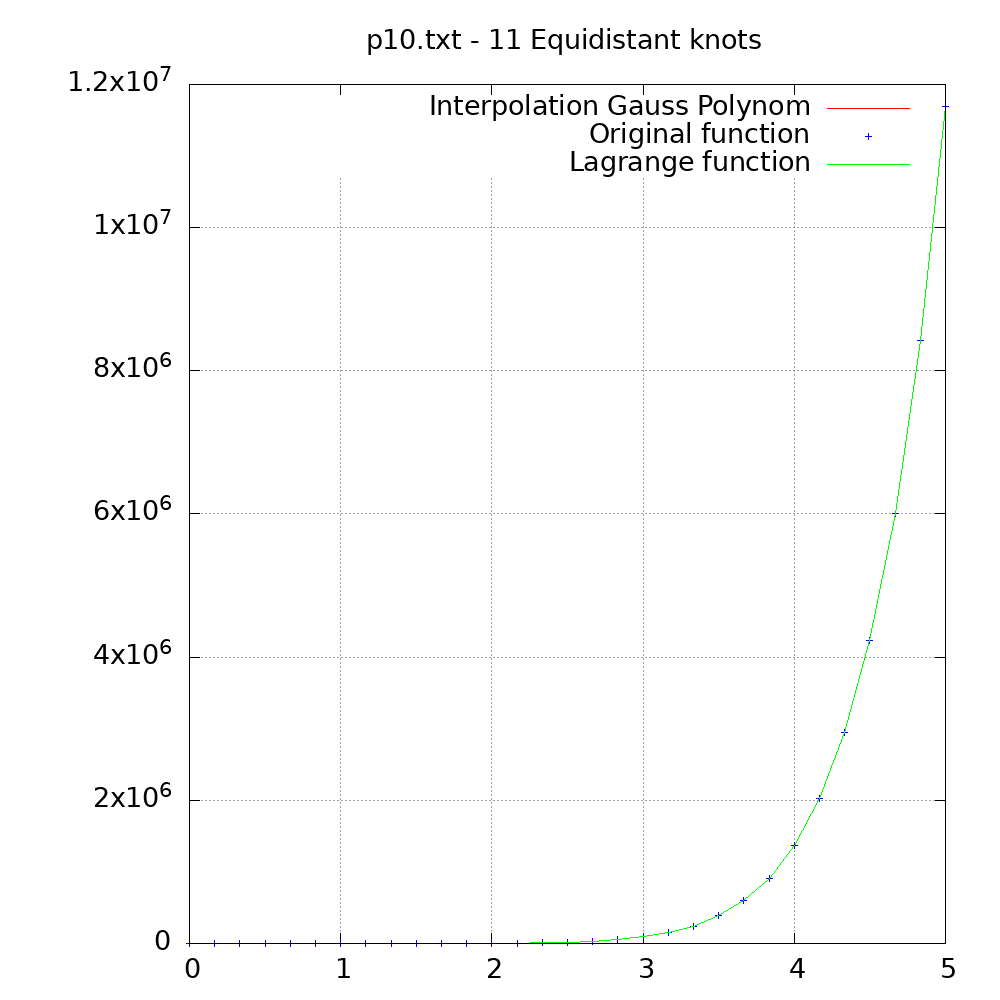
\includegraphics[scale=0.5]{Images/p10.txt.png}
        \caption{Результаты теста "Полином 10 степени" на равноудаленных узлах.}
    \end{figure}
    При этом, восстановленный полином: \\
    $11x^0 + -7.48166e-09x^1 + 1x^2 + 2x^3 + 1.13098e-07x^4 + 3x^5 + -2x^6 + -1.06963e-08x^7 + 5x^8 + -1.85583e-10x^9 + 1x^10$ \\
    Оригинальный: \\
    $11x^0 + 0x^1 + 1x^2 + 2x^3 + 0x^4 + 3x^5 + -2x^6 + 0x^7 + 5x^8 + 0x^9 + 1x^10$

    \begin{figure}
        \centering
        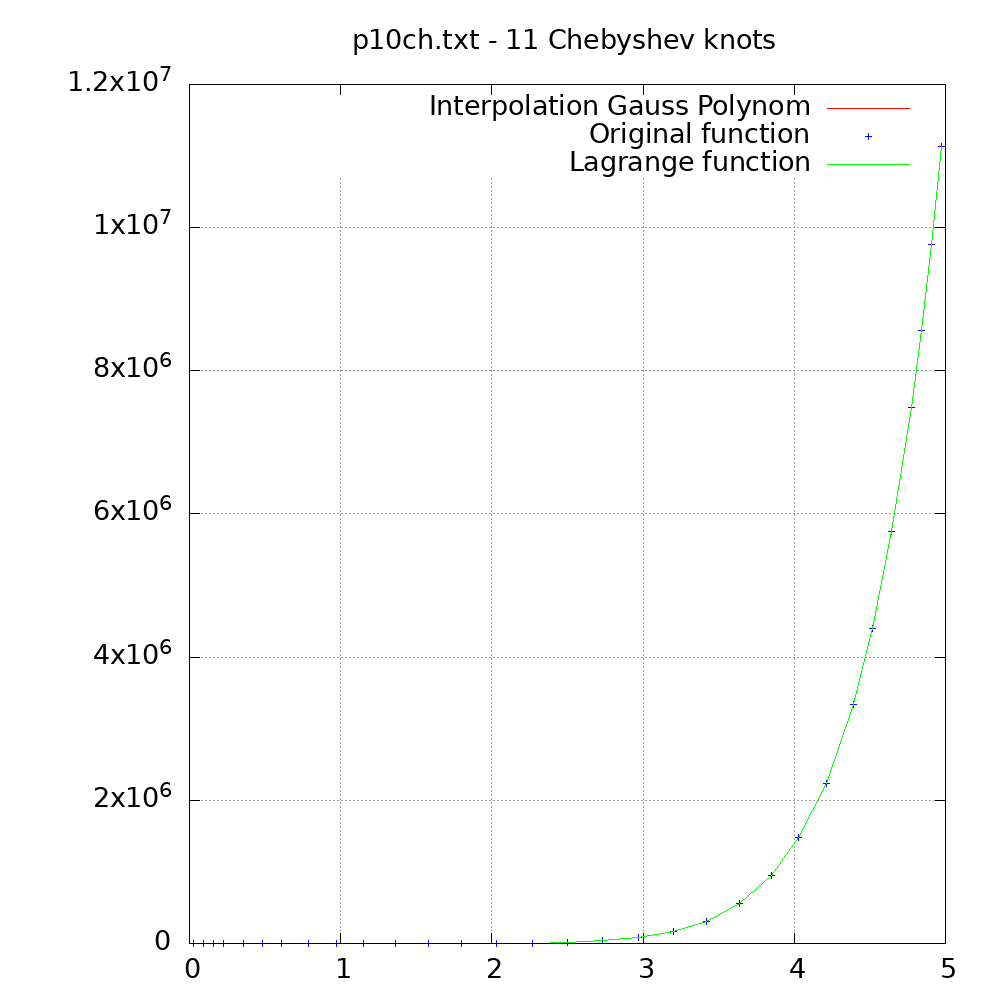
\includegraphics[scale=0.5]{Images/p10ch.txt.png}
        \caption{Результаты теста "Полином 10 степени" на Чебышёвских узлах.}
    \end{figure}
    При этом, восстановленный полином: \\
    $11x^0 + 1.09349e-09x^1 + 1x^2 + 2x^3 + -3.69267e-08x^4 + 3x^5 + -2x^6 + 4.60408e-09x^7 + 5x^8 + 8.05749e-11x^9 + 1x^10$ \\
    Оригинальный: \\
    $11x^0 + 0x^1 + 1x^2 + 2x^3 + 0x^4 + 3x^5 + -2x^6 + 0x^7 + 5x^8 + 0x^9 + 1x^10$


    \subsection{$\log(x^2 + x + 3)$.}
    \begin{figure}
        \centering
        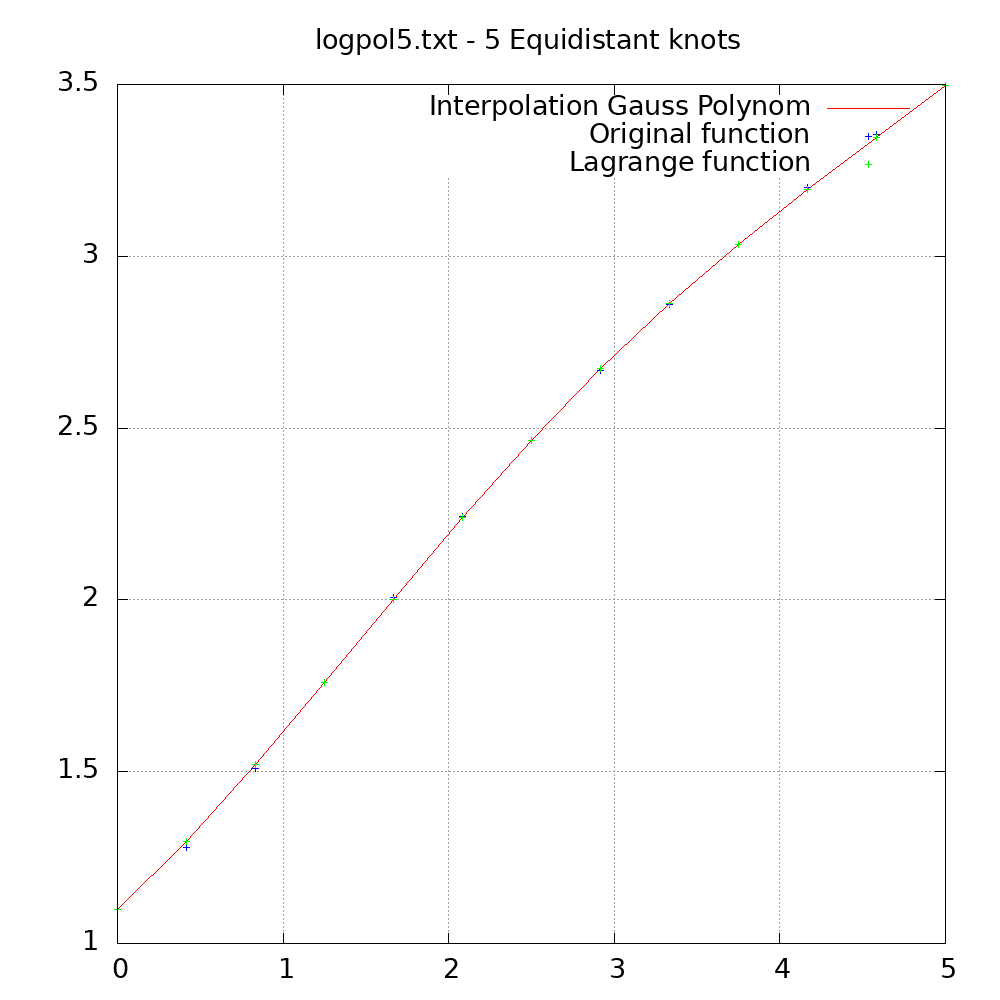
\includegraphics[scale=0.5]{Images/logpol5.txt.png}
        \caption{Результаты теста "$\log(x^2 + x + 3)$".}
    \end{figure}

    \begin{figure}
        \centering
        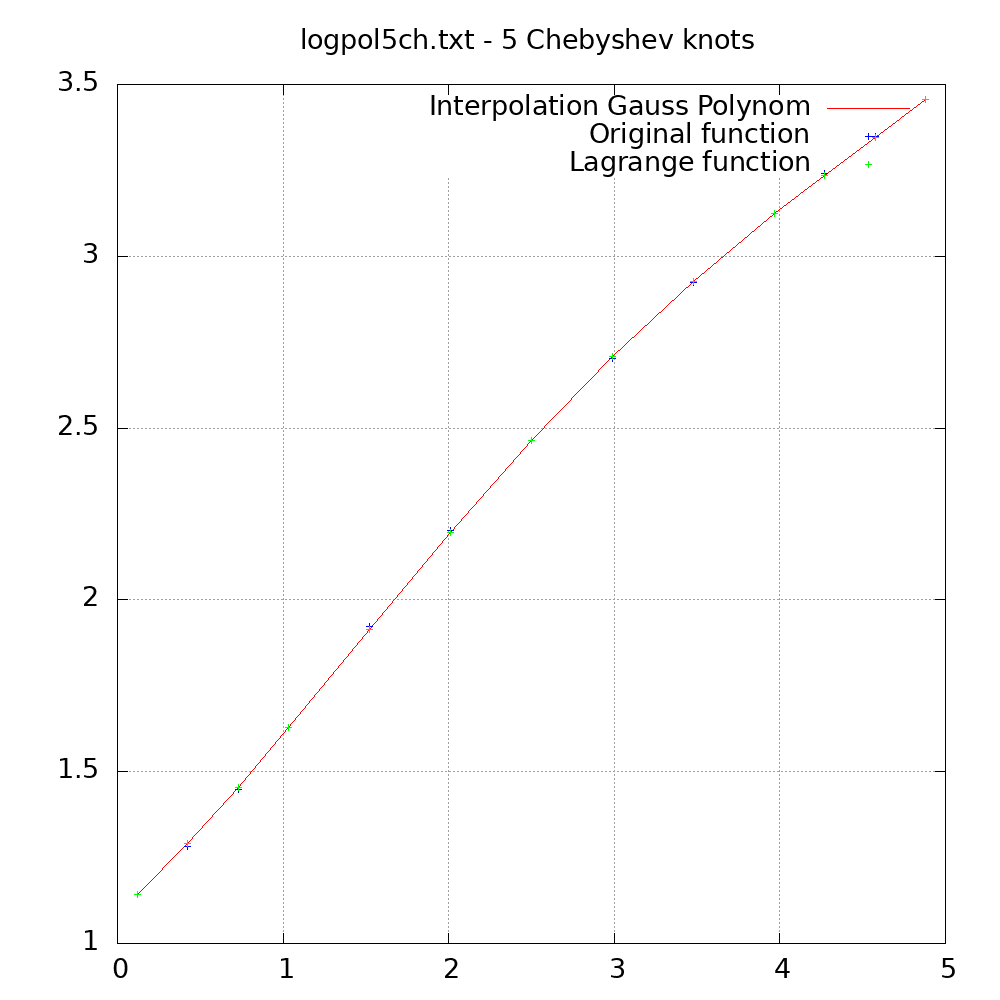
\includegraphics[scale=0.5]{Images/logpol5ch.txt.png}
        \caption{Результаты теста "$\log(x^2 + x + 3)$".}
    \end{figure}

    \begin{figure}
        \centering
        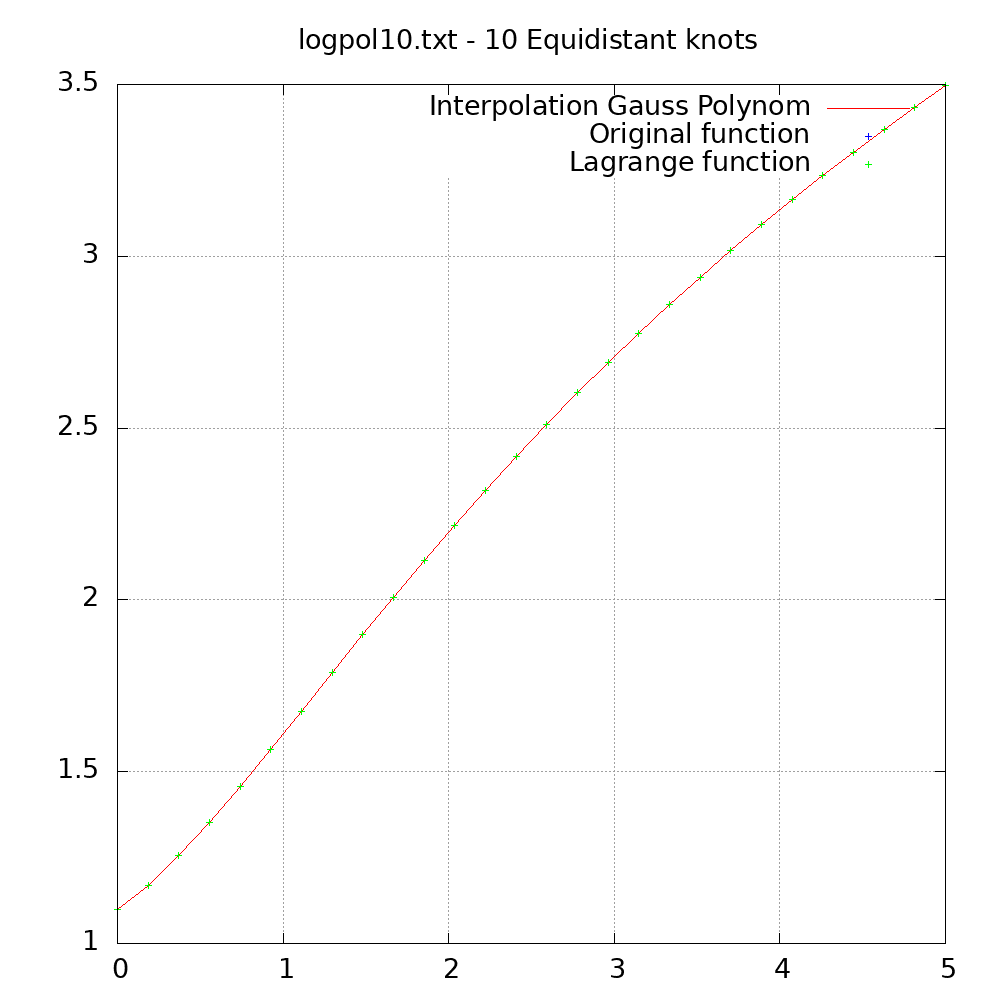
\includegraphics[scale=0.5]{Images/logpol10.txt.png}
        \caption{Результаты теста "$\log(x^2 + x + 3)$".}
    \end{figure}

    \begin{figure}
        \centering
        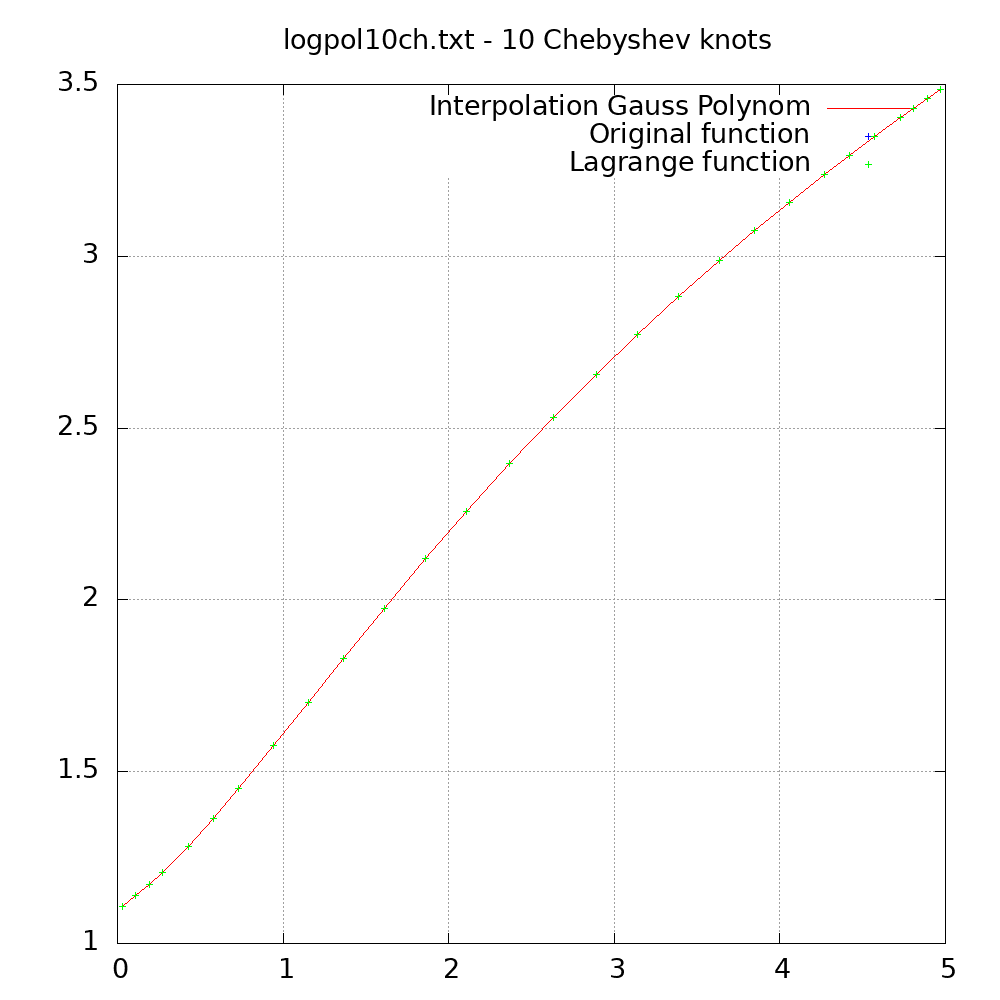
\includegraphics[scale=0.5]{Images/logpol10ch.txt.png}
        \caption{Результаты теста "$\log(x^2 + x + 3)$".}
    \end{figure}

    Как видно, на 20 узлах метод Гаусса не работает, поскольку перестаёт считать матрицу невырожденной из-за высоких степеней x.
    Тем не менее, интерполяционный многочлен Лагранжа всё ещё работает вполне исправно. \\
    На 100 узлах многочлен Лагранжа даёт сбой, но Чебышевские узлы спасают ситуацию. 
    На 1000 узлов даже Чебышёвская сеть перестает работать.

    \begin{figure}
        \centering
        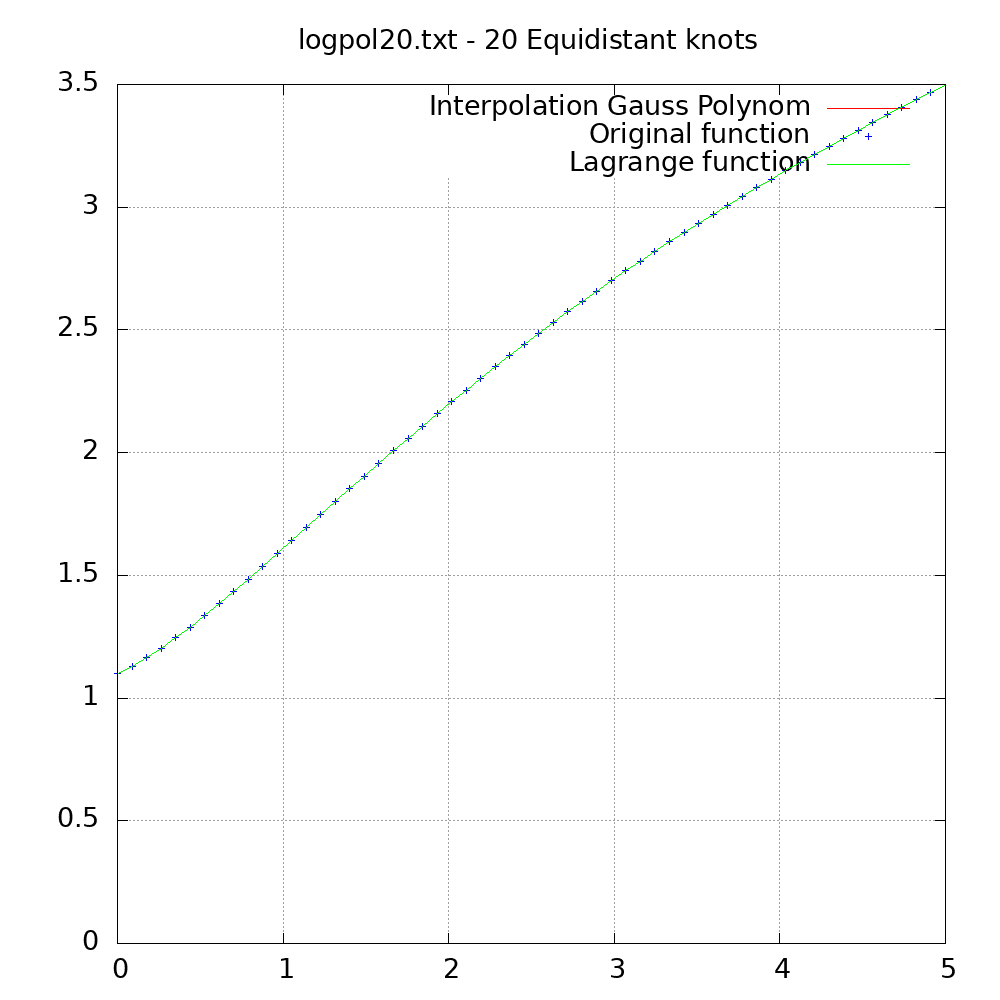
\includegraphics[scale=0.5]{Images/logpol20.txt.png}
        \caption{Результаты теста "$\log(x^2 + x + 3)$".}
    \end{figure}

    \begin{figure}
        \centering
        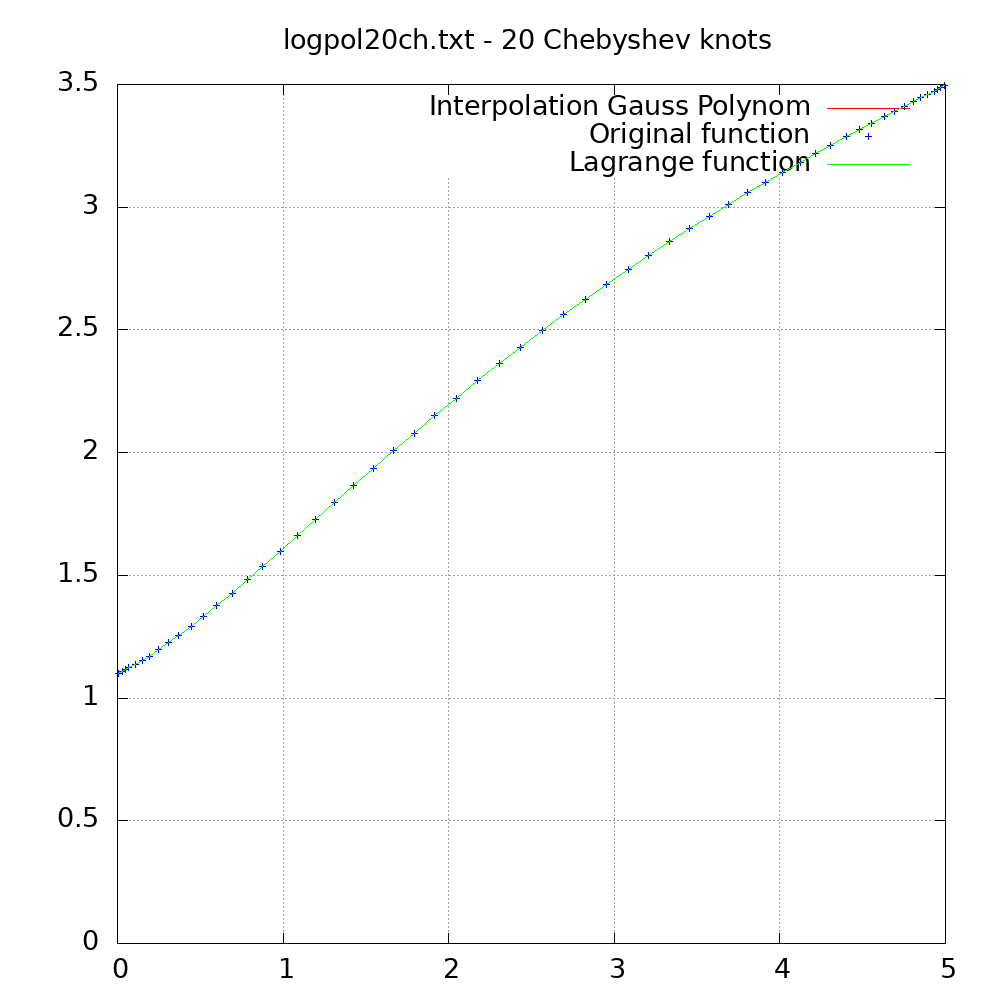
\includegraphics[scale=0.5]{Images/logpol20ch.txt.png}
        \caption{Результаты теста "$\log(x^2 + x + 3)$".}
    \end{figure}

    \begin{figure}
        \centering
        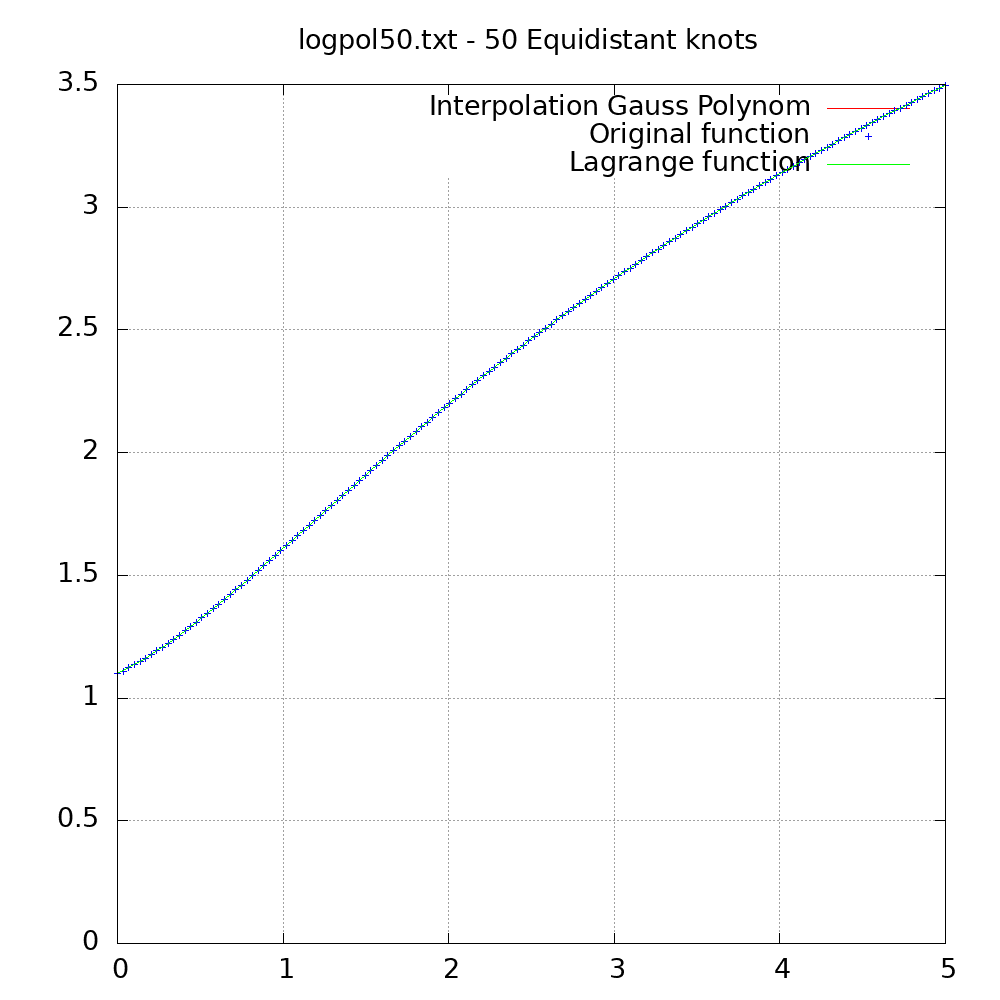
\includegraphics[scale=0.5]{Images/logpol50.txt.png}
        \caption{Результаты теста "$\log(x^2 + x + 3)$".}
    \end{figure}

    \begin{figure}
        \centering
        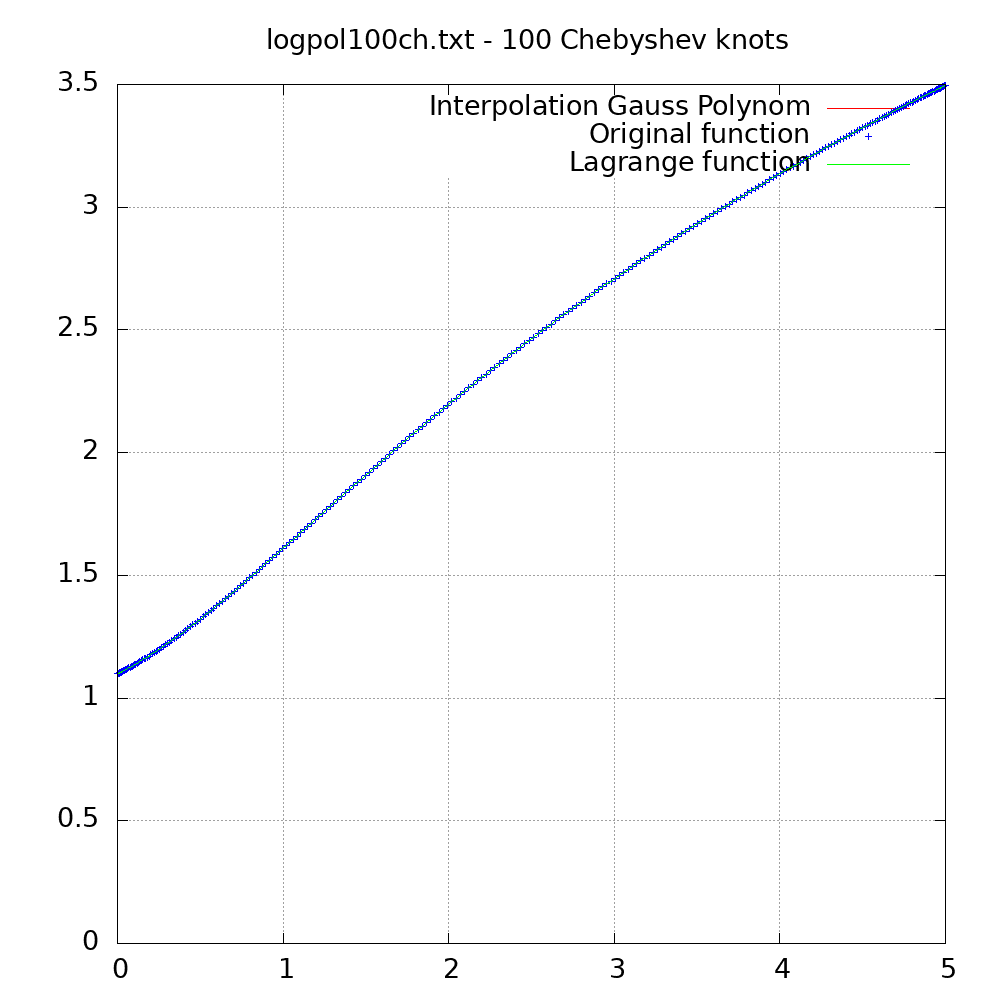
\includegraphics[scale=0.5]{Images/logpol100ch.txt.png}
        \caption{Результаты теста "$\log(x^2 + x + 3)$".}
    \end{figure}

    \begin{figure}
        \centering
        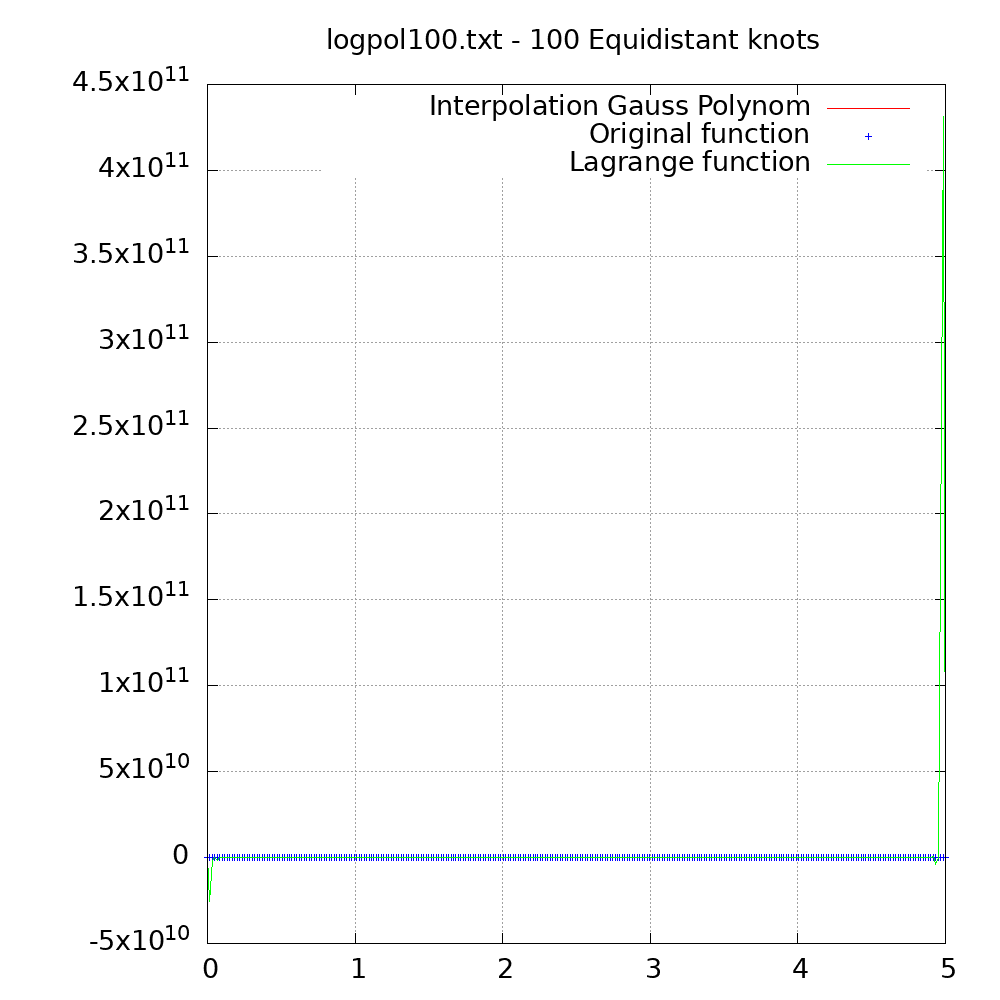
\includegraphics[scale=0.5]{Images/logpol100.txt.png}
        \caption{Результаты теста "$\log(x^2 + x + 3)$".}
    \end{figure}

    \begin{figure}
        \centering
        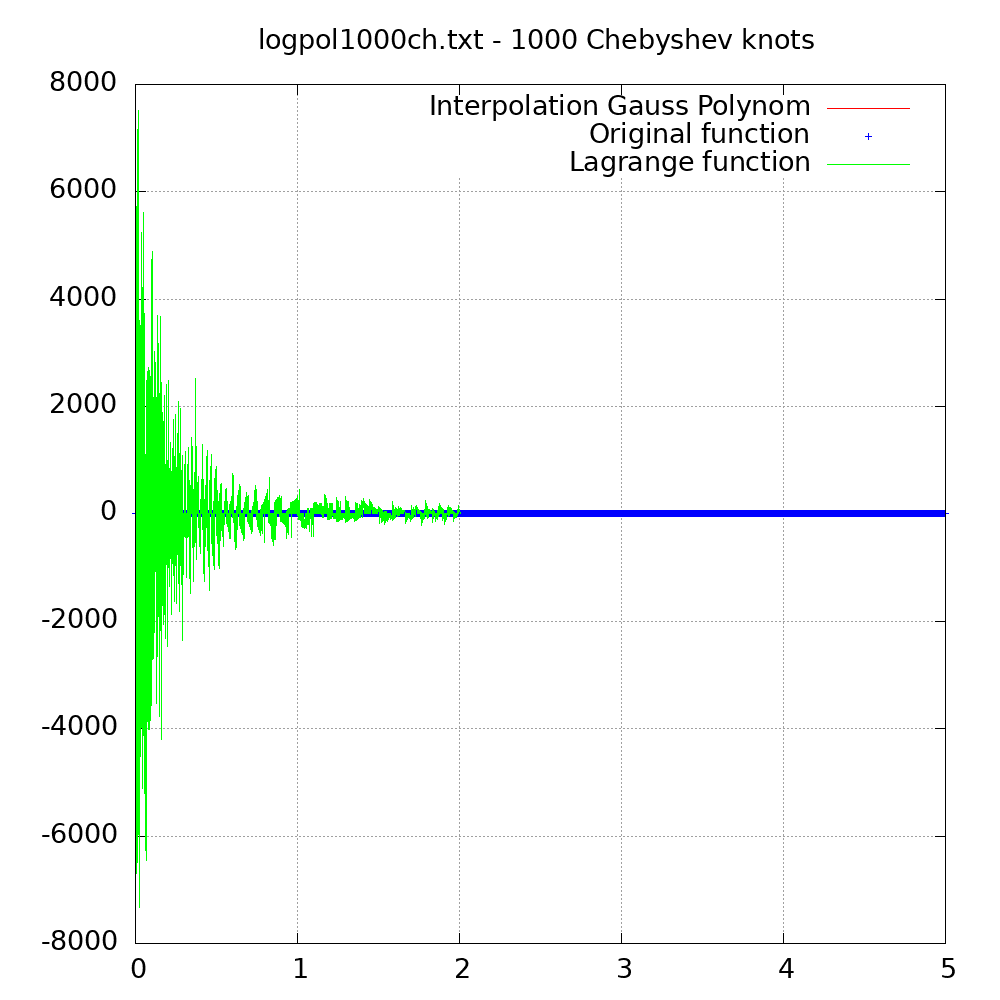
\includegraphics[scale=0.5]{Images/logpol1000ch.txt.png}
        \caption{Результаты теста "$\log(x^2 + x + 3)$".}
    \end{figure}


    \subsection{$|x|$.}

    На небольшом количестве узлов всё приблежается без проблем. Однако, уже на 20 равномерных узлах
    что-то идёт не так. Чебышёвская сеть снова спасает ситуаицю, но на 1000 узлах начинает сильно
    ассцилировать.

    \begin{figure}
        \centering
        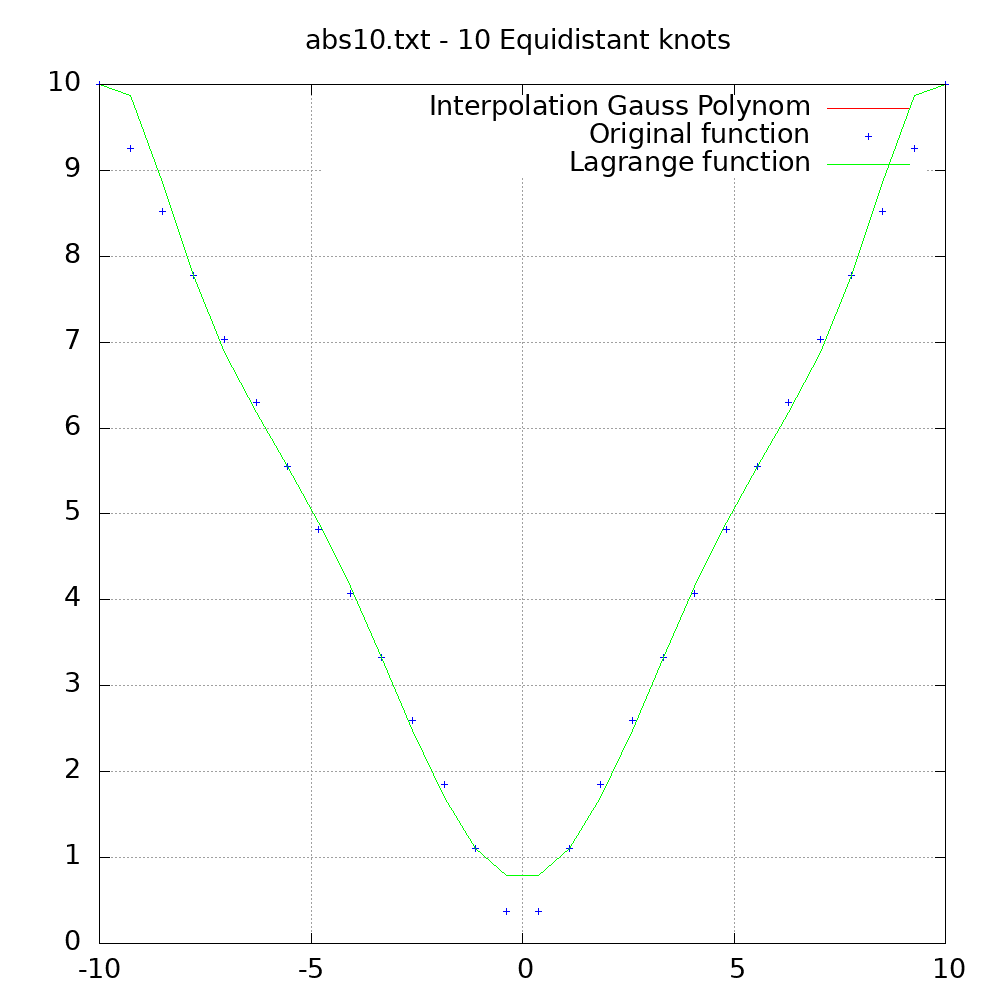
\includegraphics[scale=0.5]{Images/abs10.txt.png}
        \caption{Результаты теста "$|x|$".}
    \end{figure}

    \begin{figure}
        \centering
        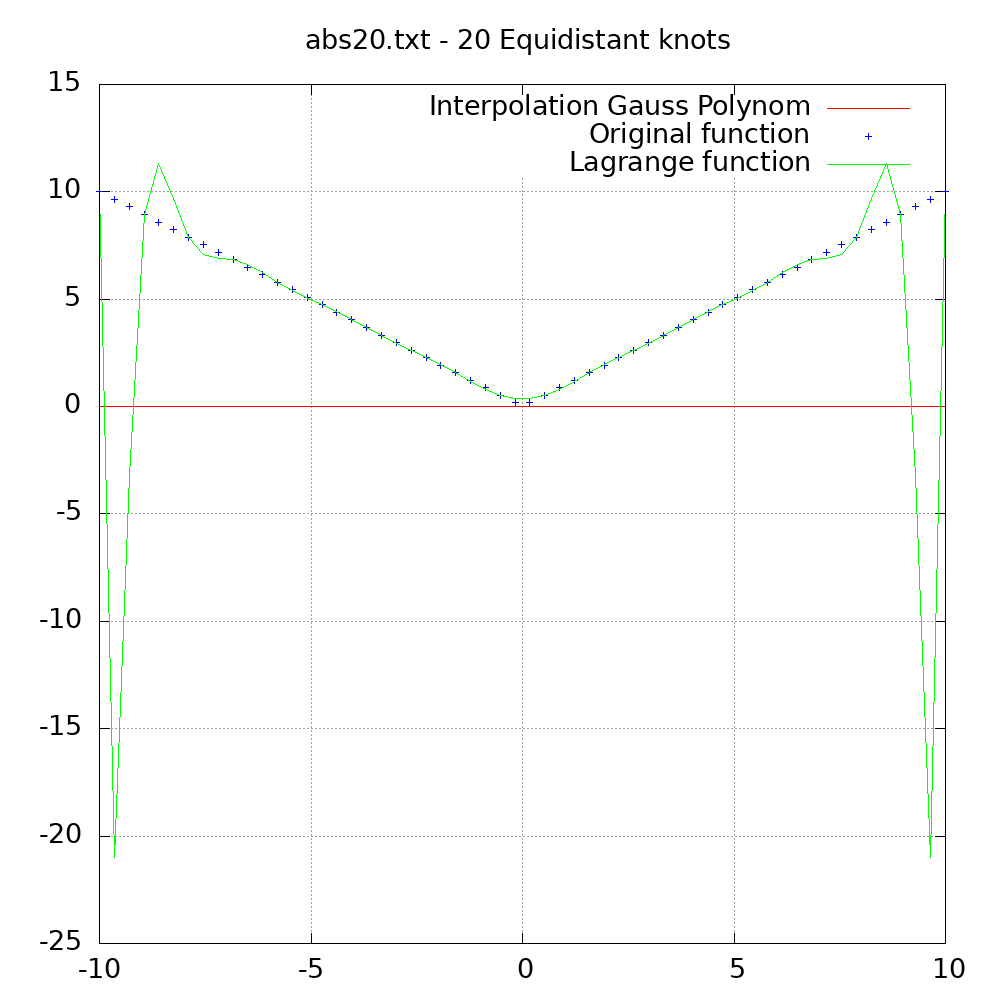
\includegraphics[scale=0.5]{Images/abs20.txt.png}
        \caption{Результаты теста "$|x|$".}
    \end{figure}
    \begin{figure}
        \centering
        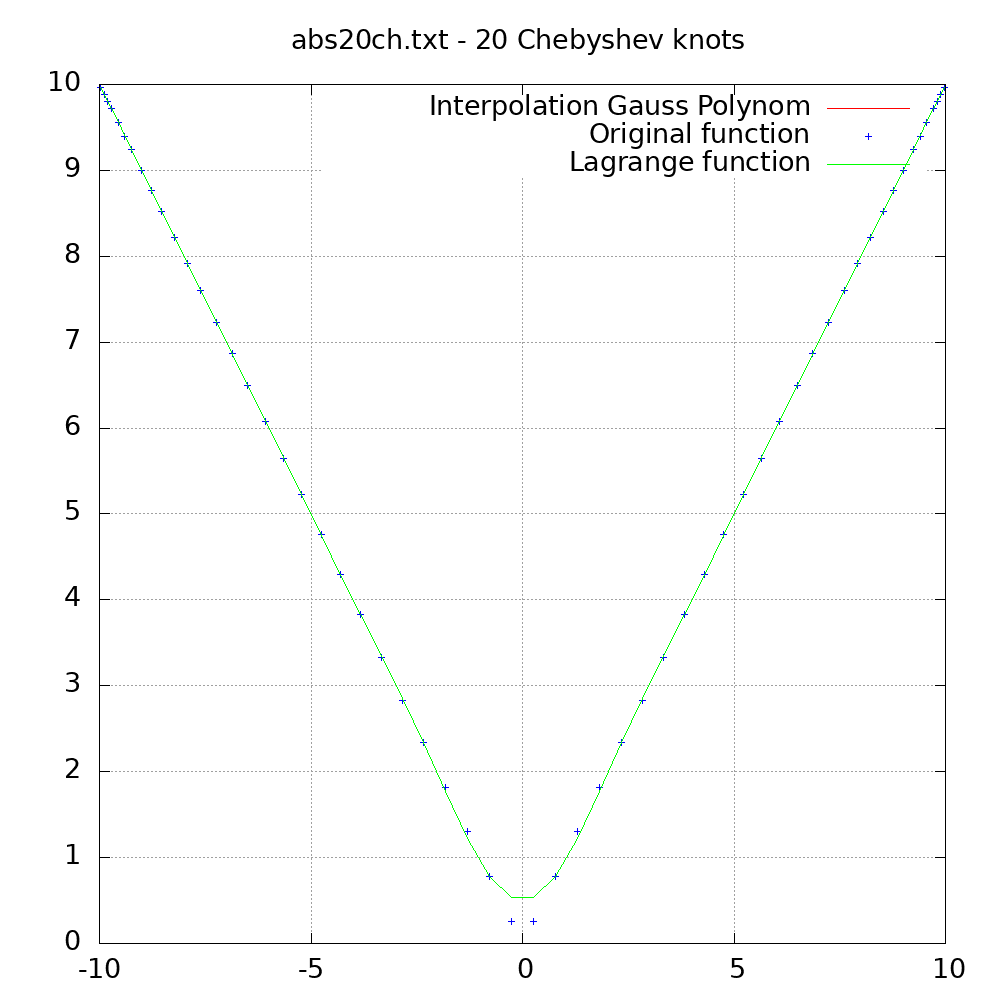
\includegraphics[scale=0.5]{Images/abs20ch.txt.png}
        \caption{Результаты теста "$|x|$".}
    \end{figure}
    \begin{figure}
        \centering
        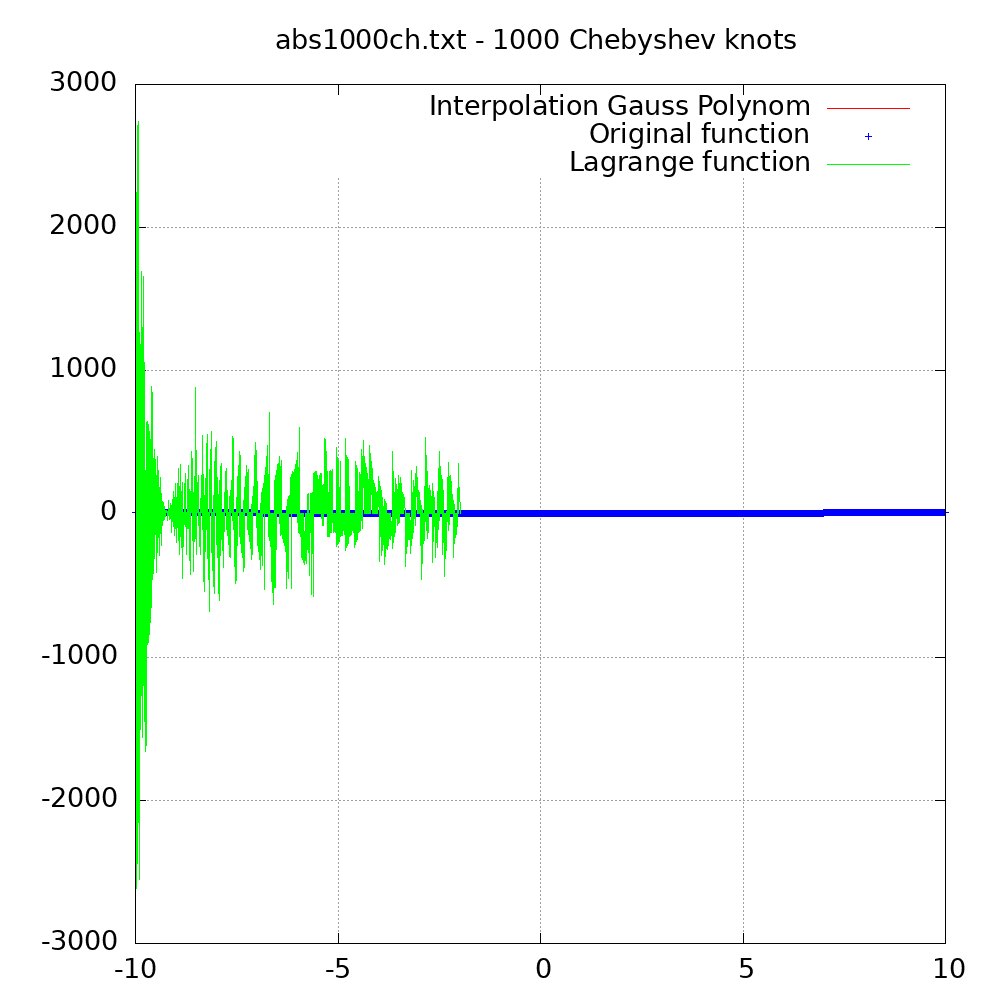
\includegraphics[scale=0.5]{Images/abs1000ch.txt.png}
        \caption{Результаты теста "$|x|$".}
    \end{figure}


    \subsection{$\frac{1}{1 + 25 x^2}$.}

    Как видно, равномерные узлы дают сбой, а Чебышёвские приближают вполне неплохо.

    \begin{figure}
        \centering
        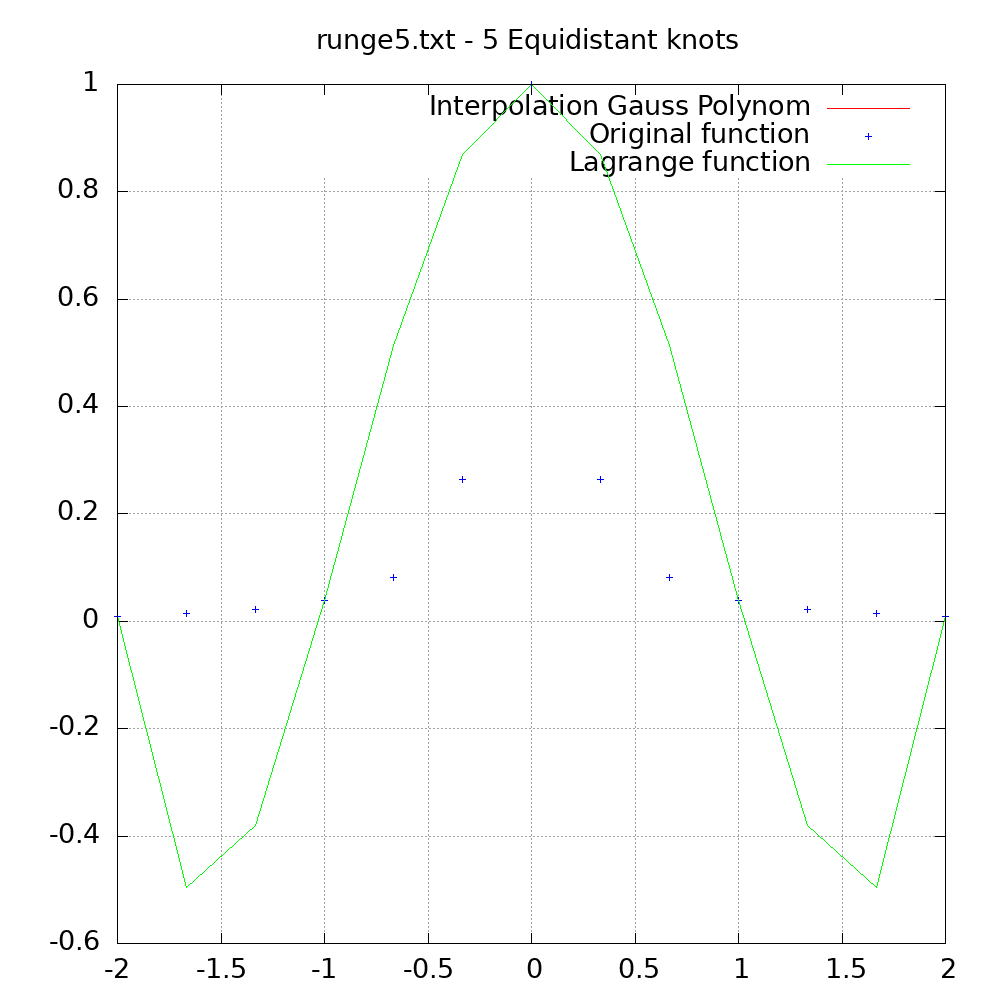
\includegraphics[scale=0.5]{Images/runge5.txt.png}
        \caption{Результаты теста "$|x|$".}
    \end{figure}
    \begin{figure}
        \centering
        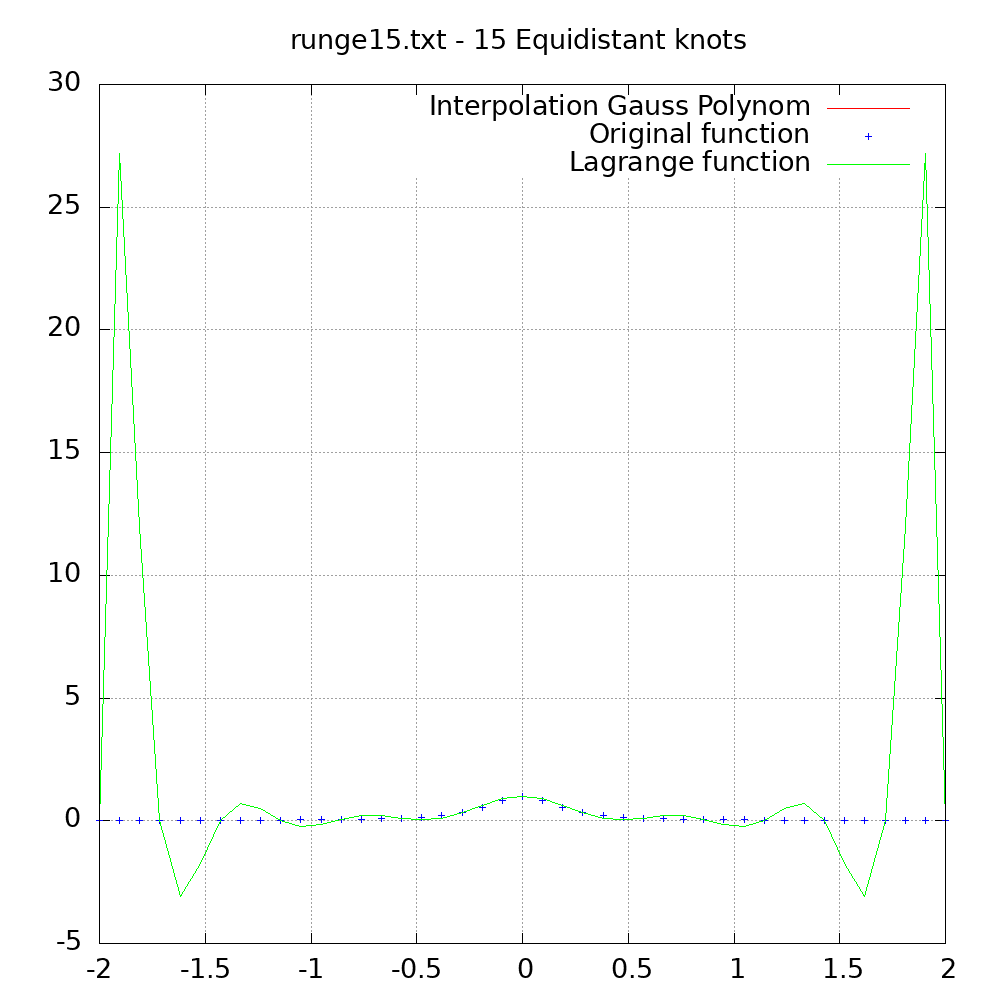
\includegraphics[scale=0.5]{Images/runge15.txt.png}
        \caption{Результаты теста "$|x|$".}
    \end{figure}
    \begin{figure}
        \centering
        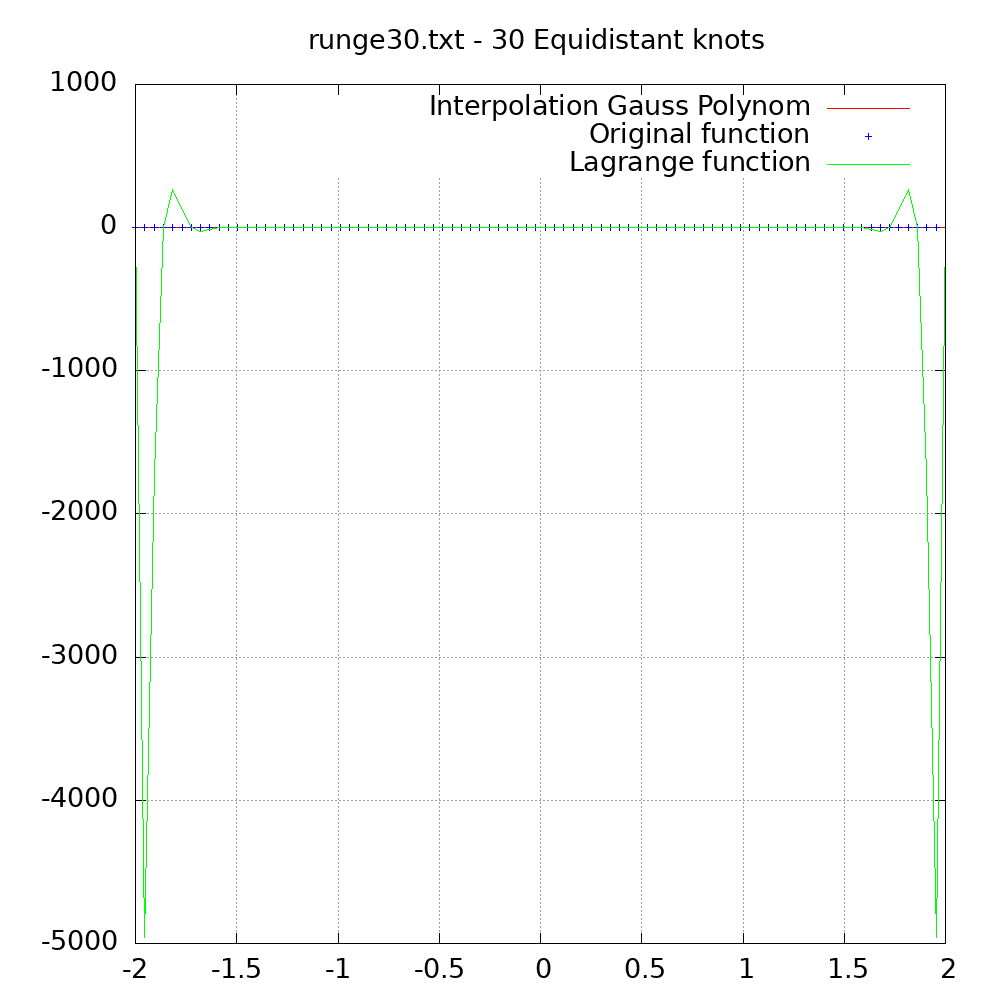
\includegraphics[scale=0.5]{Images/runge30.txt.png}
        \caption{Результаты теста "$|x|$".}
    \end{figure}

    \begin{figure}
        \centering
        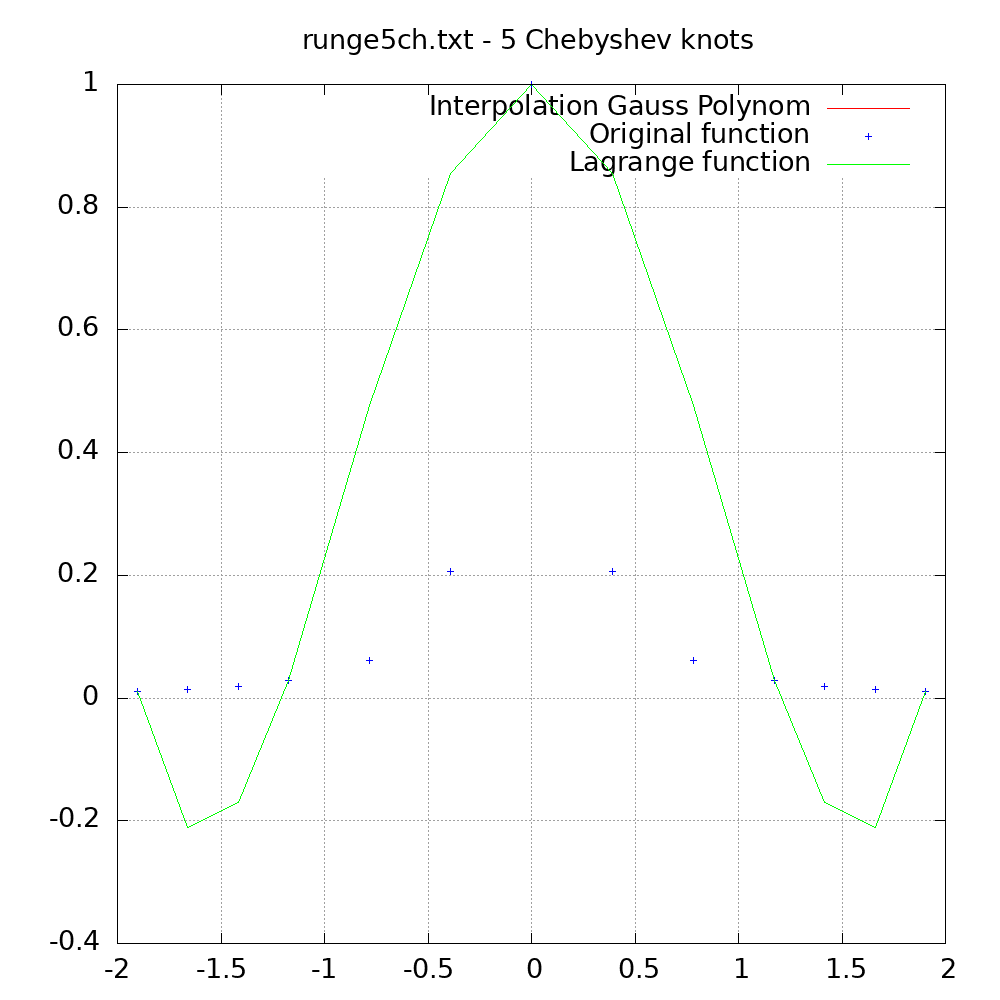
\includegraphics[scale=0.5]{Images/runge5ch.txt.png}
        \caption{Результаты теста "$|x|$".}
    \end{figure}
    \begin{figure}
        \centering
        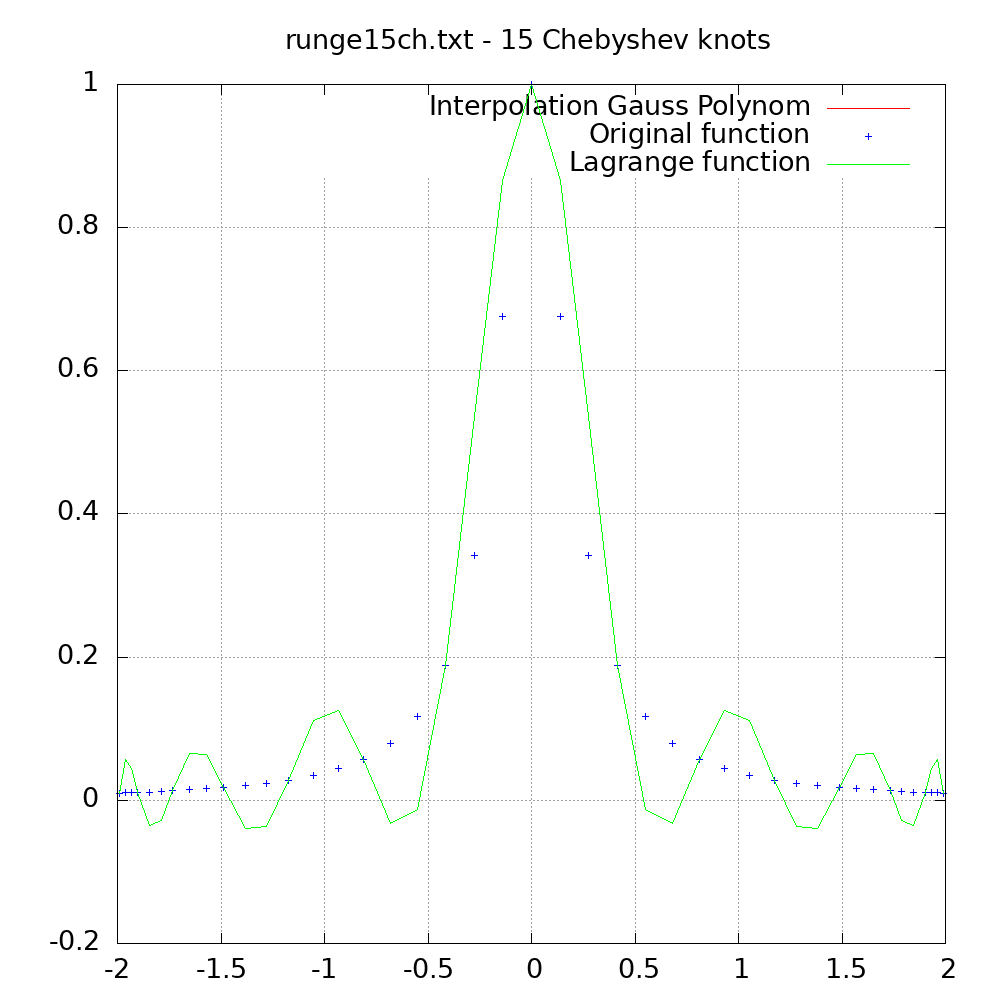
\includegraphics[scale=0.5]{Images/runge15ch.txt.png}
        \caption{Результаты теста "$|x|$".}
    \end{figure}
    \begin{figure}
        \centering
        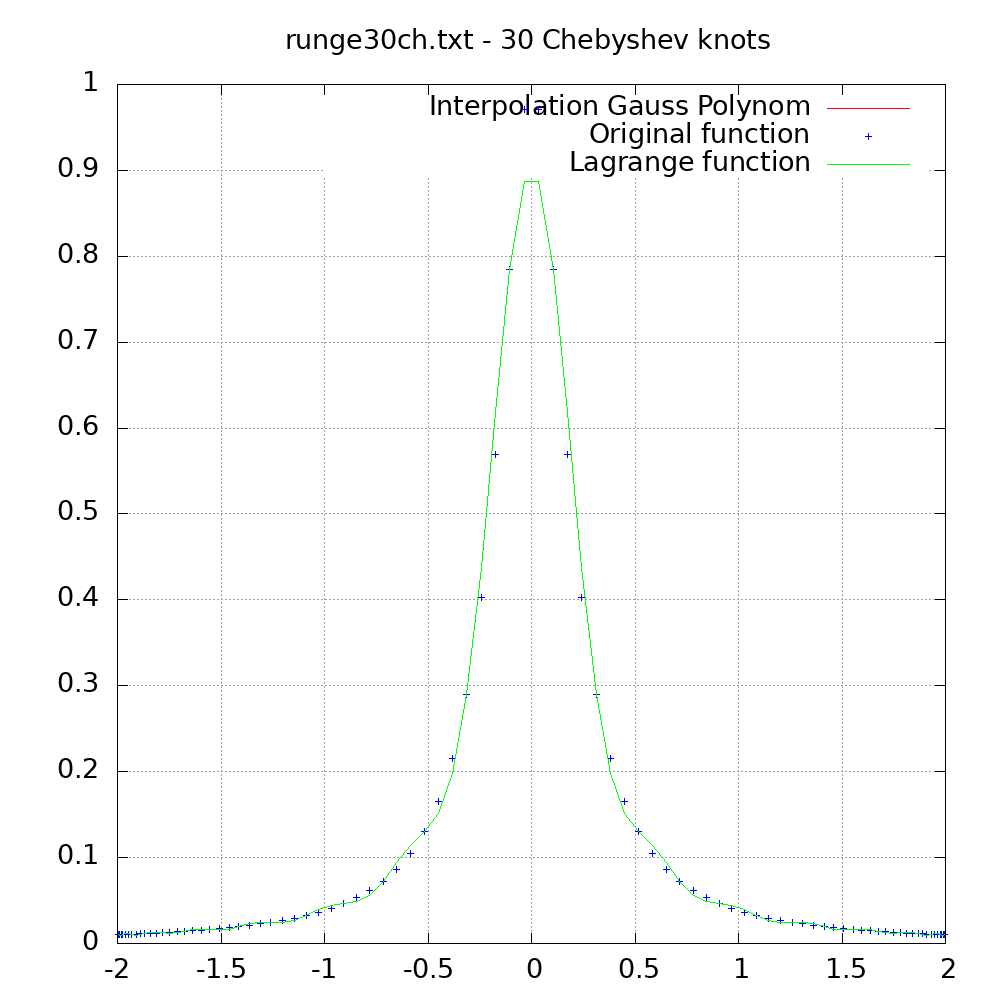
\includegraphics[scale=0.5]{Images/runge30ch.txt.png}
        \caption{Результаты теста "$|x|$".}
    \end{figure}



\end{document}